\documentclass[11pt,
			   %10pt, 
               %hyperref={colorlinks},
               aspectratio=169
               ]{beamer}
\usetheme{Singapore}

\usepackage[utf8]{inputenc}
\usepackage[T1]{fontenc}
\usepackage[american]{babel}
\usepackage{graphicx}
\usepackage{hyperref}

\usepackage[natbib=true,style=authoryear,backend=bibtex,useprefix=true]{biblatex}
\setbeamercolor*{bibliography entry title}{fg=black}
\setbeamercolor*{bibliography entry location}{fg=black}
\setbeamercolor*{bibliography entry note}{fg=black}
\setbeamertemplate{bibliography item}{}
\setbeamerfont{caption}{size=\footnotesize}
\setbeamertemplate{frametitle continuation}{}
\renewcommand*{\bibfont}{\scriptsize}
\addbibresource{bibliography.bib}

\author{Patrick Hall}
\title{Machine Learning Interpretability}
\subtitle{The Good, the Bad, and the Ugly}
\logo{
\includegraphics[height=8pt]{img/h2o_logo.png}}
\institute{\href{https://www.h2o.ai}{H\textsubscript{2}O.ai}}
\date{Aug. 1 2018}
\subject{Machine Learning Interpretability Guidance for Practitioners}

\begin{document}
	
	\maketitle
	
	\begin{frame}
	
		\frametitle{Contents}
		
		\tableofcontents{}
		
	\end{frame}

%-------------------------------------------------------------------------------
	\section{Front Matter}
%-------------------------------------------------------------------------------
	
		\begin{frame}
		
			\frametitle{Obligatory Front Matter}
			
				\begin{itemize}
					
					\item \textbf{What is interpretation?} “The	ability	to explain or to present in understandable terms to	a human.” \cite{been_kim1}
					
					\item \textbf{What is a good interpretation?} "When you can no longer keep asking why." \cite{gilpin2018explaining}
					
					\item \textbf{Why should you care?}
					\begin{itemize}
						\item Understanding of an impactful and quickly expanding set of technologies. 
						\item Addressing accidental or intentional discrimination.
						\item Preventing malicious hacking and adversarial attacks.
						\item Enabling regulatory compliance and increased financial margins.
					\end{itemize}
					
				\end{itemize}
			
		\end{frame}

%-------------------------------------------------------------------------------
	\subsection{Notation}
%-------------------------------------------------------------------------------
	
		\begin{frame}
		
			\frametitle{Notation}
			
				\begin{itemize}
					\item \textbf{Spaces}.  
					\begin{itemize}
						\item The input features come from a set  $\mathcal{X}$ contained in a \textit{P}-dimensional input space\\ (i.e. $\mathcal{X} \subset \mathbb{R}^P)$.  
						\item The output responses come from a set $\mathcal{Y}$ contained in a $C$-dimensional output space (i.e. $\mathcal{Y} \subset \mathbb{R}^C$).
					\end{itemize}	
					\bigskip	
					\item \textbf{Dataset}. A dataset $\mathbf{D}$ consists of $N$ tuples of observations:\\ $[(\mathbf{x}^{(0)},\mathbf{y}^{(0)}), (\mathbf{x}^{(1)},\mathbf{y}^{(1)}), \dots, (\mathbf{x}^{(N-1)},\mathbf{y}^{(N-1)})], \mathbf{x}^{(i)} \in \mathcal{X}, \mathbf{y}^{(i)} \in \mathcal{Y}$.\\
					\begin{itemize}
						\item The input data $\mathbf{X}$ is composed of the set of row vectors $\mathbf{x}^{(i)}$. 
						\begin{itemize}
							\item let $\mathcal{P}$ be the set of features  $\{X_0, X_1, \dots, X_{P-1}\}$, where $X_j = \left[x_{j}^{(0)}, x_{j}^{(1)}, \dots, x_{j}^{(N-1)} \right]^T$.
							\item then each $i$-th observation denoted as $\mathbf{x}^{(i)} = \left[x_0^{(i)}, x_1^{(i)}, \dots, x_{P-1}^{(i)} \right]$ is an instance of $\mathcal{P}$.
						\end{itemize}
				\end{itemize}
			\end{itemize}
		
		\end{frame}

%-------------------------------------------------------------------------------
    \subsection{Learning Problem}
%-------------------------------------------------------------------------------
	
		\begin{frame}
		
			\frametitle{Proposed Updates to the Learning Problem}
			
			\begin{figure}[htb]
				\begin{center}
					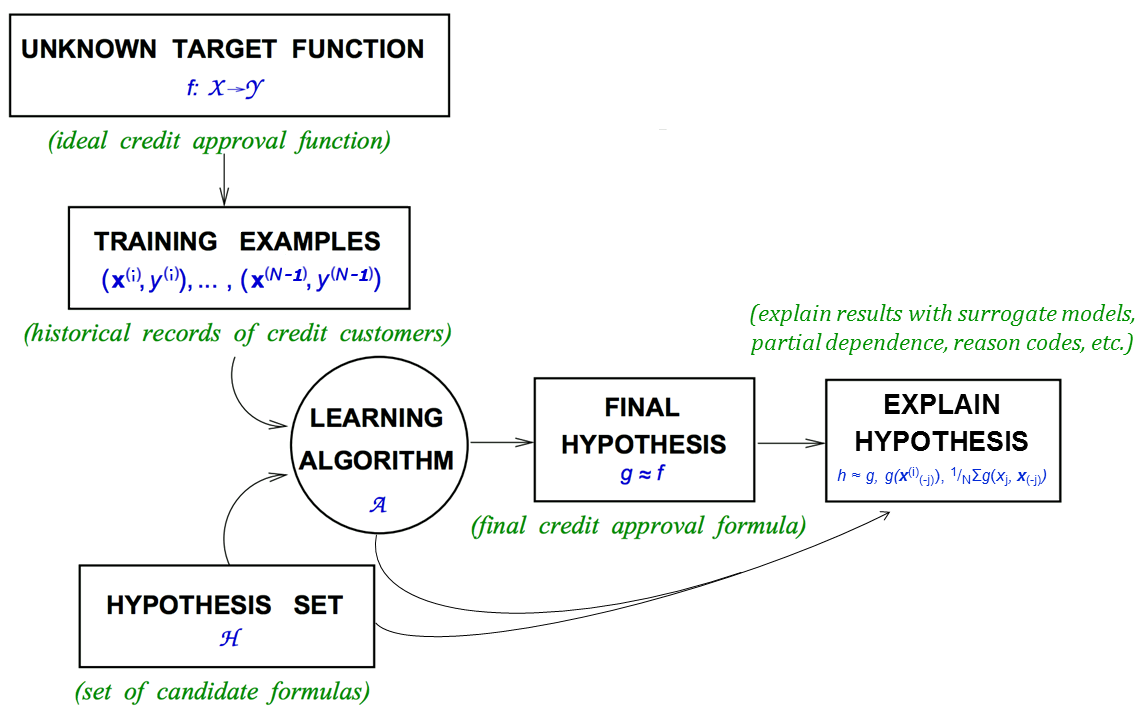
\includegraphics[height=140pt]{img/learning_problem.png}
					\label{fig:learning_problem}
				\end{center}
			\end{figure}
			
			The learning problem. Adapted from \cite{lfd}.
			
		\end{frame}

%-------------------------------------------------------------------------------
	\section{Surrogate DT}
%-------------------------------------------------------------------------------

		\begin{frame}[t]
		
			\frametitle{Surrogate Decision Trees (DT)}
			
			\begin{figure}[htb]
				\begin{center}
					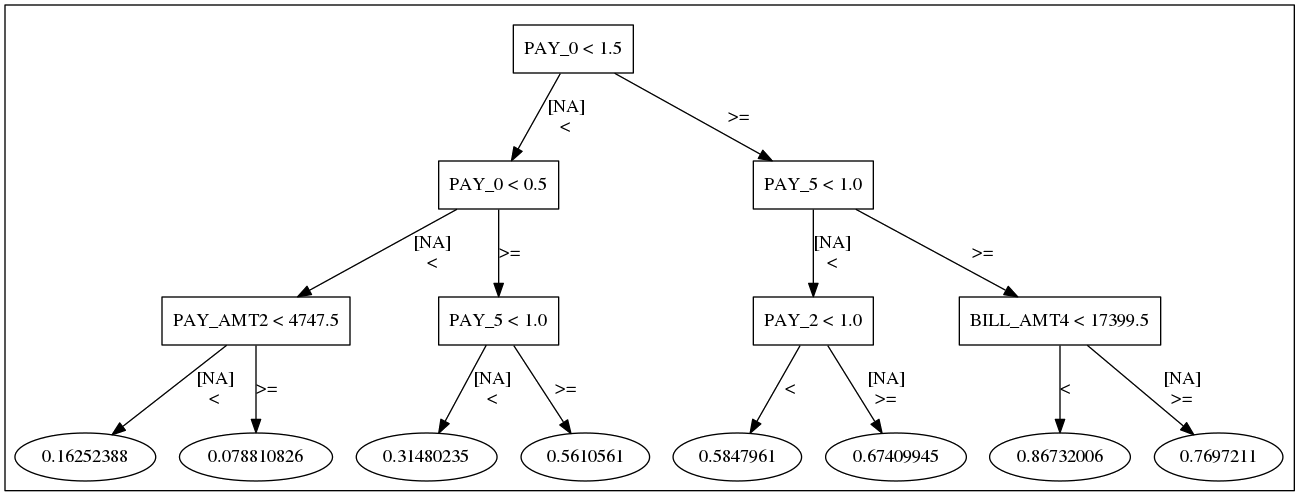
\includegraphics[height=90pt]{img/dt_surrogate.png}
					\label{fig:dt_surrogate}
					\caption{$h_{\text{tree}}$ for Taiwanese credit card data \cite{uci}, and for machine-learned GBM response function $g$.}
				\end{center}
			\end{figure}
			
			\vspace{-20 pt}
			
			\begin{itemize}
				
				\item Given a learned function $g$ and set of predictions, $g(\mathbf{X}) = \hat{\mathbf{Y}}$, a surrogate DT can be trained: $ \mathbf{X}, g(\mathbf{X}) \xrightarrow{\mathcal{A}_{\text{surrogate}}} h_{\text{tree}}$.
		
				\item $h_{\text{tree}}$ displays a low-fidelity, highly interpretable flow chart of $g$'s decision making process, and important features and interactions in $g$.	
			
			\end{itemize}
			
		\end{frame}
	
		\begin{frame}
		
			\frametitle{Surrogate Decision Trees (DT)}
			
			\begin{itemize}
				
				\item Always use error measures to assess the trustworthiness of $h_{\text{tree}}$.
	
				\item Prescribed methods (\cite{dt_surrogate1}; \cite{dt_surrogate2}) for training $h_{\text{tree}}$ do exist. In practice, straightforward cross-validation approaches are typically sufficient. 
				
				\item Comparing cross-validated error to standard training error can give an indication of the stability of the single tree model, $h_{\text{tree}}$.
				
				\item \cite{lime-sup} use local linear surrogate models, $h_{\text{GLM}}$, in $h_{\text{tree}}$ leaf nodes to increase overall surrogate model fidelity while retaining a high degree of interpretability.
				
			\end{itemize}
			
		\end{frame}

%-------------------------------------------------------------------------------
	\section{PD and ICE}
%-------------------------------------------------------------------------------

		\begin{frame}
		
			\frametitle{Partial Dependence (PD) and Individual Conditional Expectation (ICE)}
			
				\vspace{-10 pt}
			
				\begin{itemize}
					
					\item Following \cite{esl} a single feature $X_j \in \mathbf{X}$, a $P$-dimensional feature space,  and its complement set $X_{(-j)}$ (where $X_j \cup X_{(-j)} = \mathbf{X}$) is considered.
					
					\item $\text{PD}(X_j, g)$ for a given feature $X_j$ is estimated as the average of the output of the learned function $g$, where all the components of $X_j$ are set to a constant $x^{(i)}_j \in X_j$, and $\mathcal{P}_{(-j)}$ is left untouched.
					
					\item $\text{ICE}(\mathbf{x}^{(i)}_j, g)$ for a given row $\mathbf{x}^{(i)}$ and feature $X_j$ is estimated as the output of the learned function $g$ where $x^{(i)}_j$ is set to a constant $x^{(i)}_j \in X_j$ and $\mathbf{x}^{(i)} \in\mathcal{P}_{(-j)}$ are left untouched.
					
					\item PD and ICE are usually plotted over some set of interesting $x^{(i)}_j \in X_j$. 
				
				\end{itemize}
			
		\end{frame}
	
		\begin{frame}[t]
		
			\frametitle{Partial Dependence (PD) and Individual Conditional Expectation (ICE)}
		
			\begin{figure}[htb]
				\begin{center}
					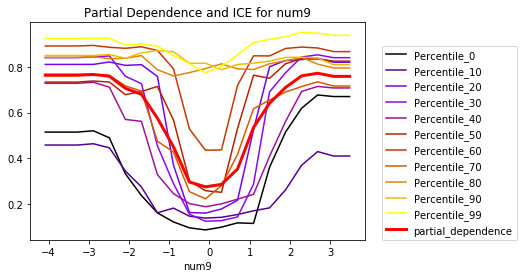
\includegraphics[height=100pt]{img/pdp_ice.png}
					\label{fig:pdp_ice}
					\caption{PD and ICE curves for $ X_j = \text{num}_9$, for known signal generating function $f(\mathbf{X}) = \text{num} _1 * \text{num}_4 + |\text{num}_8| * \text{num}_9^2 + e$, and for machine-learned GBM response function $g(\mathbf{X})$.}
				\end{center}
			\end{figure}
			
			\vspace{-10pt}
			
			Overlaying PD and ICE curves is a succinct method for describing global and local prediction behavior and can be used to detect interactions. \cite{ice_plots} 
			
		\end{frame}
	
		\begin{frame}[t]
	
			\frametitle{Partial Dependence (PD) and Individual Conditional Expectation (ICE)}
			
			\vspace{-20pt}
				
				\begin{figure}[htb]
					\begin{center}
						\label{fig:dt_surrogate_pdp_ice}
						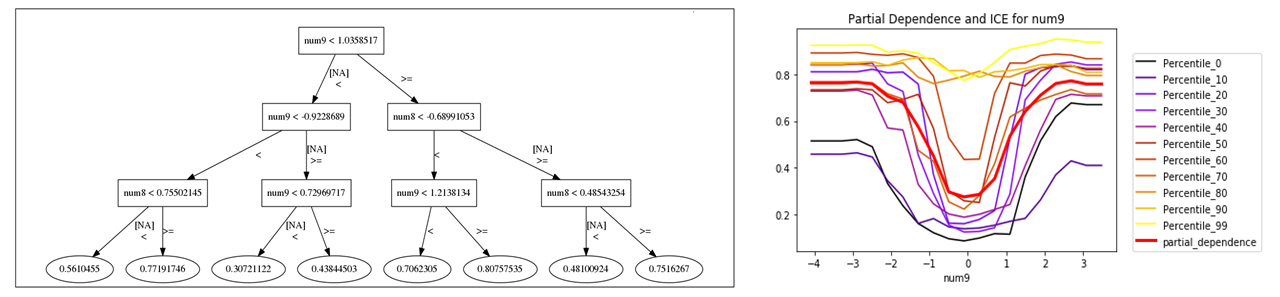
\includegraphics[height=95pt]{img/dt_surrogate2_pdp_ice2.png}
						\caption{Surrogate DT, PD, and ICE curves for $ X_j = \text{num}_9$, for known signal generating function $f(\mathbf{X}) = \text{num} _1 * \text{num}_4 + |\text{num}_8| * \text{num}_9^2 + e$, and for machine-learned GBM response function $g(\mathbf{X})$.}
					\end{center}
				\end{figure}
			
				Combining Surrogate DT models with PD and ICE curves is a convenient method for detecting, confirming, and understanding important interactions. 
	
		\end{frame}

%-------------------------------------------------------------------------------
	\section{LIME}
%-------------------------------------------------------------------------------

		\begin{frame}
		
			\frametitle{Local Interpretable Model-agnostic Explanations (LIME)}
			
				\cite{lime} defines LIME for some $x^{(i)}_j \in \mathbf{X}$:
			
				\begin{equation*}
					\begin{aligned}
						\underset{h \in \mathcal{H}}{\arg\max}\:\mathcal{L}(g, h, \pi_{\mathbf{X}}) + \Omega(h)
					\end{aligned}
				\end{equation*}
			
				Here $g$ is the function to be explained, $h$ is an interpretable surrogate model of $g$, often a linear model $h_{GLM}$, $\pi_{\mathbf{X}}$ is a weighting function over the domain of $g$, and $\Omega(h)$ limits the complexity of $h$.
			
				\vspace{5pt}
			
				Typically, $h_{GLM}$ is constructed such that $\mathbf{X}^{(*)}, g({X}^{(*)}) \xrightarrow{\mathcal{A}_{\text{surrogate}}} h_{\text{GLM}}$, where $\mathbf{X}^{(*)}$ is a generated sample, $\pi_{\mathbf{X}}$ weighs $\mathbf{X}^{(*)}$ samples by their Euclidean similarity to $x^{(i)}_j$, local feature importance is estimated using $\beta_j x^{(i)}_j$, and $L_1$ regularization is used to induce a simplified, sparse $g$. 		
			
			
		\end{frame}
	
		\begin{frame}
		
			\frametitle{Local Interpretable Model-agnostic Explanations (LIME)}
			
			\begin{itemize}
			
				\item LIME is ideal for creating low-fidelity, highly interpretable explanations for non-DT models and for neural network models trained on unstructured data, e.g. deep learning.
			
				\item Always use regression fit measures to assess the trustworthiness of LIME explanations.
			
				\item LIME can be difficult to deploy, but there are highly deployable variants. \cite{lime-sup}; \cite{h2o_mli_booklet}
			
				\item Local feature importance values are offsets from a local intercept.
				
				\begin{itemize}
					
					\item Note that the intercept in LIME can account for the most important local phenomena.
					
					\item Generated LIME samples can contain large proportions of out-of-range data that can lead to unrealistic intercept values. 
					 
				\end{itemize}
			
			\end{itemize}
			
		\end{frame}
	
		\begin{frame}[t]
		
			\begin{itemize}
		
				\item Try LIME on discretized input features and on manually constructed interactions.

				\item Use cross-validation to construct standard deviations or even confidence intervals for local variable importance values.

				\item LIME can fail, particularly in the presence of extreme nonlinearity or high-degree interactions.
		
			\end{itemize}
		
		\end{frame}

%-------------------------------------------------------------------------------
	\section{Tree Shap}
%-------------------------------------------------------------------------------

		\begin{frame}
		
			\frametitle{Tree Shap - \textit{Description}}
			
		\end{frame}
	
		\begin{frame}
		
			\frametitle{Tree Shap - \textit{Recommendations}}
			
		\end{frame}

% High fidelity

%-------------------------------------------------------------------------------
	\section{Recommendations}
%-------------------------------------------------------------------------------

		\begin{frame}
		
			\frametitle{Closing Recommendations}
			
				\begin{itemize}
					
					\item Monotonically constrained XGBoost, Surrogate DT, PD and ICE plots, and Tree Shap are a direct and open source way to create an interpretable nonlinear model.
					
					\item Global and local explanatory techniques are often necessary to explain a model.
					
					\item Use simpler low-fidelity or sparse explanations to understand more accurate and complex high-fidelity explanations.  
					
					\item Seek consistent results across multiple explanatory techniques. 
					
					\item Methods relying on generated data are sometimes unpalatable to users. They want to understand \textit{their} data.
					
					\item Surrogate models can provide low-fidelity explanations for model mechanisms in original feature spaces if $g$ is defined to include feature extraction or engineering.
					
					\item To increase adoption, production deployment of explanatory methods must be straightforward.
					
				\end{itemize}
			
			
		\end{frame}

%-------------------------------------------------------------------------------
	\section{Software}
%-------------------------------------------------------------------------------

		\begin{frame}

			\frametitle{Software Examples and Resources}
			
			\textbf{Comparison of Explanatory Techniques on Simulated Data:}\\
			\href{https://github.com/h2oai/mli-resources/tree/master/lime_shap_treeint_compare}{https://github.com/h2oai/mli-resources/tree/master/lime\_shap\_treeint\_compare}\\
			
			\vspace{10pt}
		
			\textbf{In-depth Explanatory Technique Examples:}\\
			\href{https://github.com/jphall663/interpretable_machine_learning_with_python}{
			https://github.com/jphall663/interpretable\_machine\_learning\_with\_python}\\
			
			\vspace{10pt}
			
			\textbf{"Awesome" Machine Learning Interpretability Resource List:}\\
			\href{https://github.com/jphall663/awesome-machine-learning-interpretability}{https://github.com/jphall663/awesome-machine-learning-interpretability}
			
		\end{frame}

%-------------------------------------------------------------------------------
%	References
%-------------------------------------------------------------------------------


	\begin{frame}[t, allowframebreaks]
	
		\frametitle{References}
		
		\printbibliography
		
	\end{frame}

\end{document}